\section{Dafny}
Dafny consists out of 4 different projects. DafnyDriver, DafnyPipleline, DafnyRuntime and the DafnyServer. Most important was the DafnyServer for this project. It had been forked to allow extensions which were merged back into the master branch of Microsoft. 
\subsection{Overview}
Dafny itself does not verify programs, but does the translation into boogie code. Boogie does mostly the same, it can translate the code to different prove engines. In addition, it can be configured to do the verification slightly different. One of the prove engines, which was used for this project, is Z3. This engine can verify if a logical formula can be proven. If a prove is found, it can also be viewed, which was important to produce counter examples, were the prove was negated. 
In addition, the DafnyServer is part of Dafny and allows caching and the opportunity to not start a new process for each verification.\newline 
\begin{figure}[H]
	\centering
	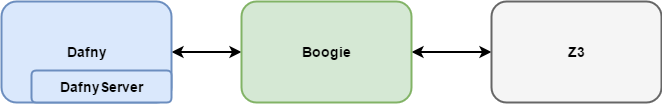
\includegraphics[width=0.8\textwidth]{img/dafny_overview}
	\caption{Interaction between Dafny, Boogie and Z3}
	\label{fig:dafny_overview}
\end{figure}
\subsection{DafnyServer API}
The DafnyServer is a simple console application which allows proofing Dafny source files. To verify documents, they are sent over the standard input. Results are obtained from the standard output. The verification task needs to be in JSON format, see \ref{verificationtaskinterface}, and is sent base64 encoded. By default, the server only supports the verbs verify, quit and selftest. Verbs are sent first, followed by a newline \textbackslash{n}. They may be proceeded by a verification task and the end string \textbf{[[DAFNY-CLIENT: EOM]]}. 
\paragraph{Verb explanation:}
\begin{itemize}
	\item \textbf{verify} needs a verification task and returns the output from the verification
	\item \textbf{quit} stops the server
	\item \textbf{selftest} execute some simple verification.
\end{itemize}
\subsubsection{Verification Task Interface}\label{verificationtaskinterface}
The verification task must use the following structure. \newline
\begin{lstlisting}[language=json,firstnumber=1]
{
  args : [],
  filename : "c:\\DEV\\Dafny\\test.dfy",
  source : "method Main() {  assert 4 < 3; }",
  sourceIsFile : false
}
\end{lstlisting}
\subsubsection{DafnyServer Example}
\textbf{Sample Request}
The base64 encoded string is the verification task from above. 
The following request examples will only show the Dafny program and not how it is sent encoded. 
\begin{lstlisting}[language={},backgroundcolor=\color{background},basicstyle=\scriptsize\ttfamily]
verify
eyJhcmdzIjpbXSwiZmlsZW5hbWUiOiJjOlxcREVWXFxEYWZueVxcdGVzdC5kZnkiLCJzb3VyY2Ui
OiJtZXRob2QgTWFpbigpIHsgIGFzc2VydCAxIDwgMzsgfSIsInNvdXJjZUlzRmlsZSI6ZmFsc2V9
[[DAFNY-CLIENT: EOM]]
\end{lstlisting}
\textbf{Sample Response}
\begin{lstlisting}[language={},backgroundcolor=\color{background},basicstyle=\scriptsize\ttfamily]
Verifying Impl$$_module.__default.Main ...
  [1 proof obligation]  error
c:\DEV\Dafny\test.dfy(1,26): Error: assertion violation
Execution trace:
    (0,0): anon0

Verification completed successfully!
[SUCCESS] [[DAFNY-SERVER: EOM]]
\end{lstlisting}
The result is plain text. There is currently no possibility to get a JSON response. Because of that, it is necessary to parse and extract the most important parts manually. 
\subsubsection{symbols}
To support refactoring in the Dafny Visual Studio Code plugin, symbol information was needed. All fields, methods and classes inside a file along with their information about position, references and usage have to be accessible. To support this, the DafnyServer was extended. A new verb "symbols" was introduced. This collects various information about the symbol table of the input file and returns it as JSON. 
\newline\newline
\textbf{Request}
\begin{lstlisting}[language=dafny]
class BankAccountUnsafe {
  var balance: int;
  constructor() modifies this { 
    balance := 10;
  }

  method withdraw(amount: int) 
    modifies this
  requires amount >= 0 {   
    balance := balance - amount; 
  } 
}   

method test() { 
  var a := new BankAccountUnsafe(); 
  a.withdraw(9);  
}   
\end{lstlisting}
\textbf{Response}
\begin{lstlisting}[language=json,firstnumber=1]
[
  ....
  {
    "Call" : null,
    "Column" : 3,
    "EndColumn" : null,
    "EndLine" : null,
    "EndPosition" : null,
    "Ensures" : [],
    "Line" : 3,
    "Module" : "_module",
    "Name" : "_ctor",
    "ParentClass" : "BankAccountUnsafe",
    "Position" : 49,
    "References" : [{
        "Column" : 12,
        "Line" : 15,
        "MethodName" : "test",
        "Position" : 265,
        "ReferencedName" : "_ctor"
      }
    ],
    "Requires" : [],
    "SymbolType" : "Method"
  }, {
    "Call" : null,
    "Column" : 9,
    "EndColumn" : null,
    "EndLine" : null,
    "EndPosition" : null,
    "Ensures" : [],
    "Line" : 6,
    "Module" : "_module",
    "Name" : "withdraw",
    "ParentClass" : "BankAccountUnsafe",
    "Position" : 114,
    "References" : [{
        "Column" : 5,
        "Line" : 16,
        "MethodName" : "test",
        "Position" : 296,
        "ReferencedName" : "withdraw"
      }
    ],
    "Requires" : ["amount >= 0"],
    "SymbolType" : "Method"
  }, {
    "Call" : null,
    "Column" : 6,
    "EndColumn" : null,
    "EndLine" : null,
    "EndPosition" : null,
    "Ensures" : null,
    "Line" : 2,
    "Module" : "_module",
    "Name" : "balance",
    "ParentClass" : "BankAccountUnsafe",
    "Position" : 32,
    "References" : [{
        "Column" : 5,
        "Line" : 4,
        "MethodName" : "balance",
        "Position" : 85,
        "ReferencedName" : "balance"
      }, {
        "Column" : 3,
        "Line" : 10,
        "MethodName" : "balance",
        "Position" : 190,
        "ReferencedName" : "balance"
      }, {
        "Column" : 14,
        "Line" : 10,
        "MethodName" : "balance",
        "Position" : 201,
        "ReferencedName" : "balance"
      }
    ],
    "Requires" : null,
    "SymbolType" : "Field"
  }
  ....
]

\end{lstlisting}
\subsubsection{counterExample}
To show counter examples in Visual Studio Code, it was necessary to extend the server by an additional feature, which returns a counter example. To verb is called \textbf{counterExample} and uses the same payload as verify. It also needs to verify the program first, but calculates the counter model if a proof fails. This calculation can be quite complex and therefore needs a lot of time to perform.  
\textbf{Request}
\begin{lstlisting}[language=dafny]
method Abs(x: int) returns (y: int)
ensures y >= 0 {
  return x;
}
\end{lstlisting}
\textbf{Response}
\begin{lstlisting}[language=json,firstnumber=1]
{
  "States" : [{
      "Column" : 0,
      "Line" : 0,
      "Name" : "<initial>",
      "Variables" : [{
          "CanonicalName" : "((- 1))",
          "Name" : "x",
          "RealName" : null,
          "Value" : "((- 1))"
        }, {
          "CanonicalName" : "(**y#0)",
          "Name" : "y",
          "RealName" : null,
          "Value" : "(**y#0)"
        }
      ]
    }, {
      "Column" : 16,
      "Line" : 3,
      "Name" : "c:\\DEV\\Dafny\\abs.dfy(3,16): initial state",
      "Variables" : [{
          "CanonicalName" : "((- 1))",
          "Name" : "x",
          "RealName" : null,
          "Value" : "((- 1))"
        }, {
          "CanonicalName" : "(**y#0)",
          "Name" : "y",
          "RealName" : null,
          "Value" : "(**y#0)"
        }
      ]
    }, {
      "Column" : 13,
      "Line" : 4,
      "Name" : "c:\\DEV\\Dafny\\abs.dfy(4,13)",
      "Variables" : [{
          "CanonicalName" : "((- 1))",
          "Name" : "x",
          "RealName" : null,
          "Value" : "((- 1))"
        }, {
          "CanonicalName" : "((- 1))'1",
          "Name" : "y",
          "RealName" : null,
          "Value" : "((- 1))'1"
        }
      ]
    }
  ]
}

\end{lstlisting}
\subsubsection{version}
The command returns the version of the Dafny. 
\textbf{Request}
\begin{lstlisting}[language={},backgroundcolor=\color{background},basicstyle=\scriptsize\ttfamily]
version
[[DAFNY-CLIENT: EOM]]
\end{lstlisting}
\textbf{Response}
\begin{lstlisting}[language={},backgroundcolor=\color{background},basicstyle=\scriptsize\ttfamily]
VERSION:1.9.16
Verification completed successfully!
[SUCCESS] [[DAFNY-SERVER: EOM]]
\end{lstlisting}
